%-------------- Hertz -----------------------
\section{Hertz method} \label{hertz}
The Hertz method is the application of the Hertzian model of elastic contact to the initial stage of the loading curve \cite{Hertz}. 
It can be used either to estimate the modulus if the tip radius is known or vice versa, depending what information is available.

\begin{figure}[h]
  \centering
  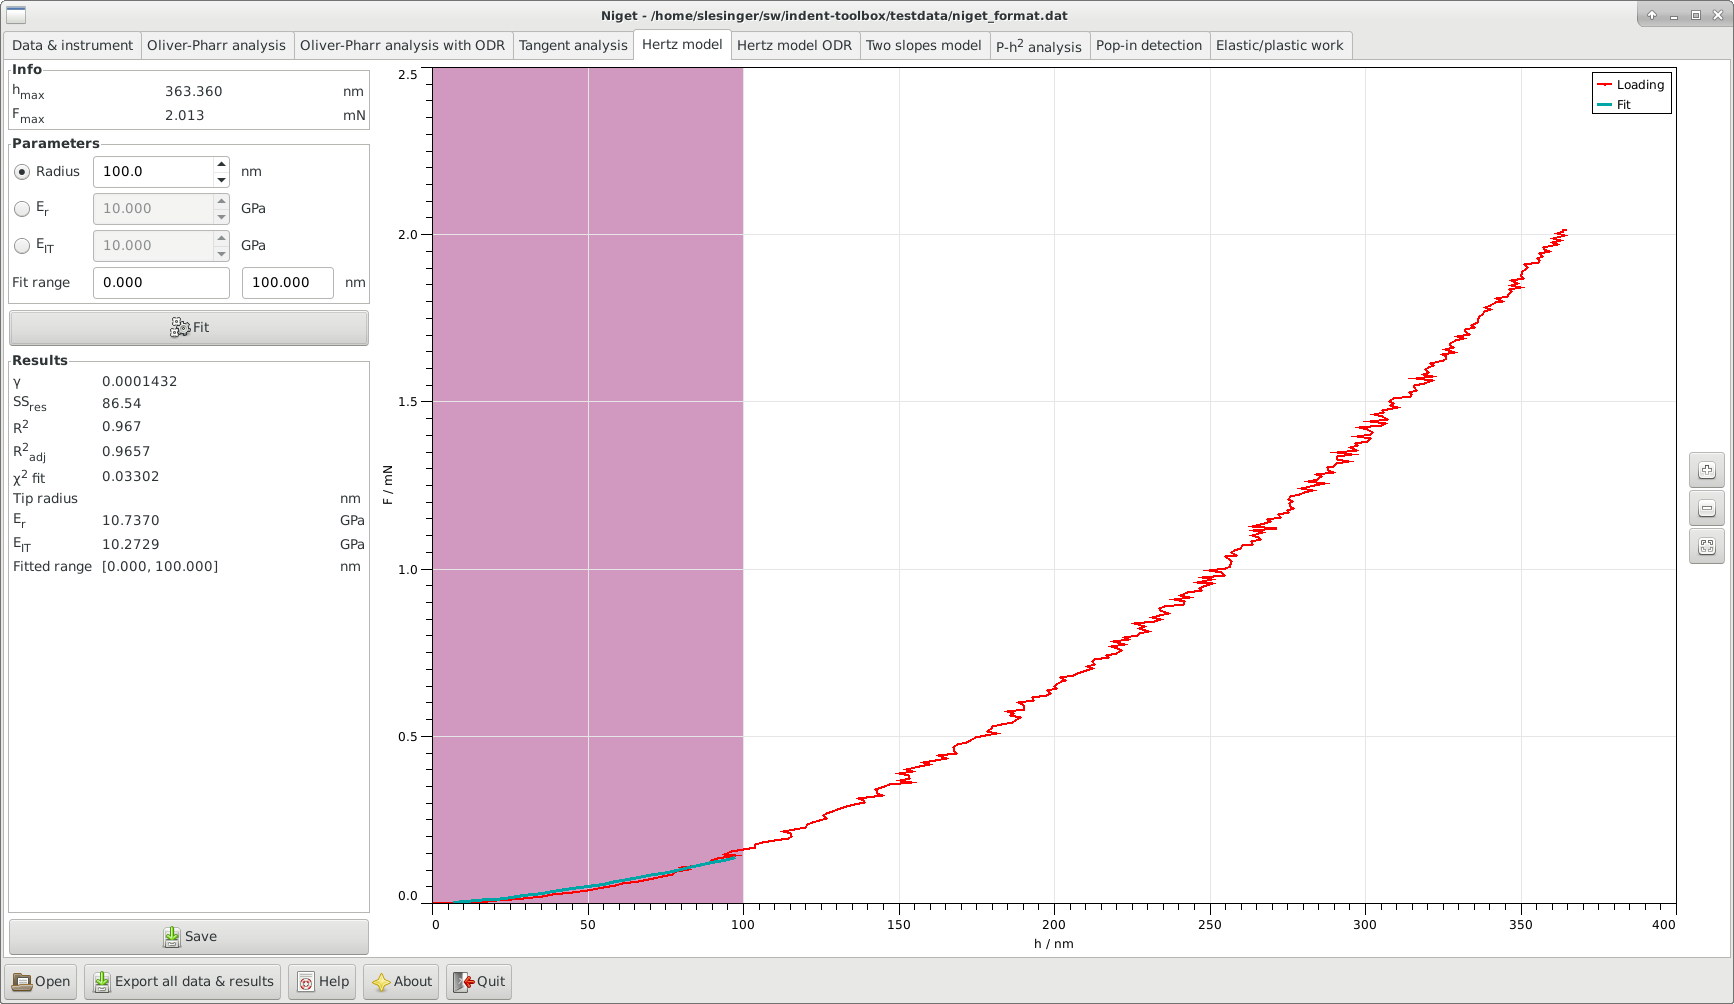
\includegraphics[width=\textwidth]{images/screen-hertz}
  \caption{Hertzian model analysis}
\end{figure}

\subsection{Window}
The window consists of several blocks:
\begin{itemize}
 \item \emph{Info} displays the maximum depth and force during the indentation
 \item \emph{Parameters} shows the selected range in nm. 
        \begin{itemize}
           \item[-] The input variable can be chosen to be either the tip radius, the reduced modulus or the indentation modulus and its value should be set accordingly.
           \item[-] The fitting range can be selected either using the mouse or typing in the range entries. The range must be chosen so that the behavior remains elastic and the fit adequate.
        \end{itemize}
 \item \emph{Fit} button, see section \ref{hertz_calc} for details of the calculation.
 \item \emph{Results} displays the results and the ranges used for the fitting procedure. 
       The variables are described in detail in section \ref{hertz_calc}.
% \item \emph{Uncertainties} show the uncertainty analysis window, see section \ref{hertz_unc}.
 \item \emph{Save} save parameters and results to given file. 
 \item \emph{Graph} display the unloading curve and the fitted curves.  Stepwise zooming/unzooming can be performed by selecting a range with the mouse and pressing the \emph{Zoom}/ \emph{Unzoom} buttons. The graph is restored to its original size by the \emph{Restore} button.
\end{itemize}

\subsection{Procedure} \label{hertz_calc}
\begin{enumerate} 
 \item 
The Hertzian model predicts for the contact between sphere and halfspace the following shape of the loading curve
\begin{equation} \label{eq:hertzfit}
F = a h^{3/2},  
\end{equation}
with 
\begin{equation}
a = \frac43 \Er \sqrt{R}.
\end{equation}
This is fitted using ordinary least squares with an additional intercept possible, see section \ref{ls:fit32}.
\item
If the tip radius is given, the contact modulus is calculated as 
\begin{equation}
\Er = \frac34 \frac{a}{\sqrt{R}}.
\end{equation}
For a comparison with Young's modulus found in literature the indentation modulus $E_{IT}$ \eqref{eq:Eit} is useful

\item
If the reduced modulus is given, the tip radius is calculated as
\begin{equation}
R =  \left(\frac34 \frac{a}{\Er}\right)^2
\end{equation}
\item
If the indentation reduced modulus is given, the material parameters $\nu$, $\nui$ and $\Ei$ are used to convert it to the reduced modulus
\begin{equation}
\Er=\left(\frac{1-\nui^2}{\Ei}+\frac{1-\nu^2}{\Eit}\right)^{-1}.
\end{equation}
from which the tip radius can be calculated as in the previous step.
\end{enumerate}
